\subsection{Integrales dobles en recintos generales}

Cuando hablamos de recintos generales,
nos referimos a recintos no rectangulares.

Se distinguen dos casos:
\begin{itemize}
    \item El recinto en \(x\) es un intervalo e \(y\) en función de \(x\) \(f(x)\)
    \item Al revés: En \(x\) tenemos funciones \(f(y)\) y los valores de \(y\) son un intervalo
\end{itemize}

Para operar estas integrales es necesario:

\begin{enumerate}
    \item Graficar el recinto
    \item Determinar intersecciones
    \item Plantear integral y operar
\end{enumerate}

\subsection{Ejemplo}

Calcular volumen para superficie \(z = x + 2y\),
en el recinto delimitado por \(y = x^{2}\) e \(y = x + 2\).

Primero,
graficamos recinto:

\begin{figure}[H]
    \centering
    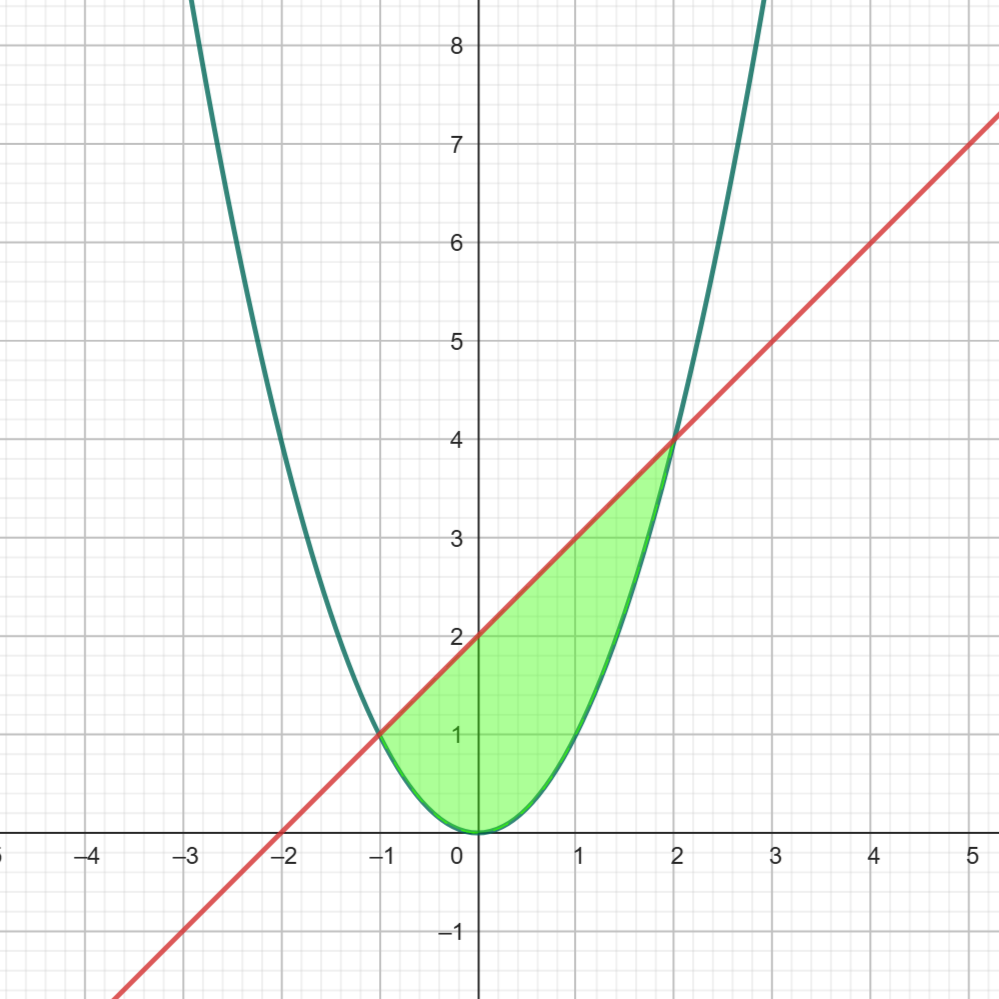
\includegraphics[scale=.9]{./img/01.png}
    \caption{Recinto}
\end{figure}

Determinamos intersecciones en \(x\):

\begin{align*}
    x^{2} = x + 2                     \\
    x^{2} - x = 2                     \\
    (x-\frac{1}{2})^{2} = \frac{9}{4} \\
    |x-\frac{1}{2}| = \frac{3}{2}     \\
    x = \frac{1}{2} \pm \frac{3}{2}   \\
    x = 2 \land x = x = -1            \\
\end{align*}

Planteamos integral:

\begin{align*}
    \int_{-1}^{2} \int_{x^{2}}^{x+2}[ x + 2y ]\,dy \,dx
\end{align*}

Resolvemos primera integral:

\begin{align*}
    \int_{x^{2}}^{x+2} x + 2y \,dy & = \int_{x^{2}}^{x+2} x \,dy + \int_{x^{2}}^{x+2} 2y \,dy \\
                                   & = xy|_{x^{2}}^{x+2} + y^{2}|_{x^{2}}^{x+2}               \\
                                   & = x^{2} + 2x - x^{3} + (x+2)^{2} - x^{4}                 \\
                                   & = x^{2} + 2x - x^{3} + x^{2} + 2x + 4 - x^{4}            \\
                                   & = -x^{4} - x^{3} + 2x^{2} + 4x + 4                       \\
\end{align*}

Operamos segunda integral.
Como vemos, si operamos primero la dependiente,
queda un polinomio en función de la otra para el final:

\begin{gather*}
    \int_{-1}^{2} -x^{4} - x^{3} + 2x^{2} + 4x + 4 \,dx = \left.-\frac{x^{5}}{5} - \frac{x^{4}}{4} + \frac{2x^{3}}{3} + 2x^{2} + 4x\right|_{-1}^{2} = \\
    = -\frac{2^{5}}{5} - \frac{2^{4}}{4} + \frac{2\cdot2^{3}}{3} + 2\cdot2^{2} + 8 + \frac{(-1)^{5}}{5} + \frac{(-1)^{4}}{4} - \frac{2(-1)^{3}}{3} - 2(-1)^{2} + 4 = \\
    = -\frac{32}{5} - 4 + \frac{16}{3} + 8 + 8 - \frac{1}{5} + \frac{1}{4} + \frac{2}{3} - 2 + 4 = \\
    = \frac{67}{5} + \frac{1}{4} = \\
    = \boxed{\frac{263}{20}} \\
\end{gather*}

\subsection{Ejemplo 2}

Resolver \(\int\!\int2\,dx\,dy\) para recinto \(R = \left\{y\leq x^{2}, y\geq0, x\geq0, x+y-2<0, x-y-1\leq0\right\}\)

Por las condiciones \(y\geq0, x\geq0\),
determinamos que tiene que estar en el primer cuadrante.

Despejamos las dos desigualdades restantes:

\begin{align*}
    x+y-2 & < 0   \\
    y     & < 2-x \\
\end{align*}

\begin{align*}
    x-y-1 & \leq 0   \\
    y     & \geq x-1 \\
\end{align*}

Entonces, el recinto tiene que estar delimitado por:

\begin{align*}
    \begin{cases}
        y     < 2-x \\
        y \geq x-1  \\
        y\leq x^{2}
    \end{cases}
\end{align*}

Graficamos:

\begin{figure}[H]
    \centering
    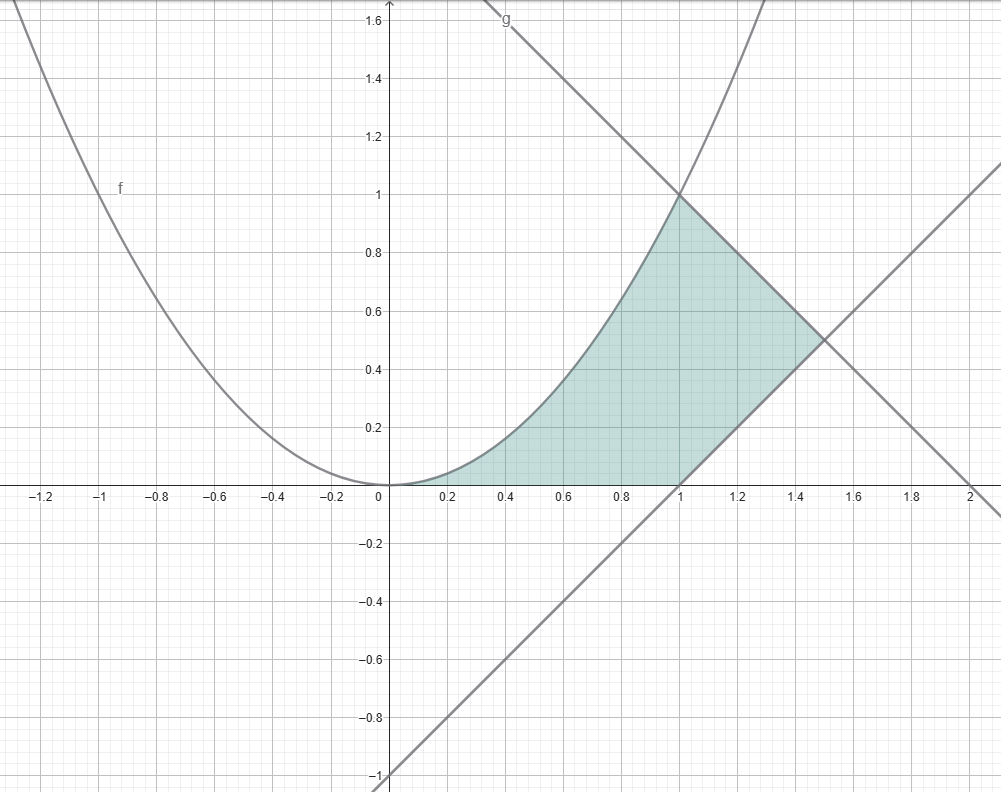
\includegraphics[scale=.5]{./img/02-recinto2.png}
    \caption{Recinto 2}
\end{figure}

Por propiedad de las integrales dobles,
podemos dividir el recinto en dos subrecintos, 
de manera tal que:

\begin{align*}
    &R_1 = [0,1] \times [0,x^{2}] &&\text{y} &R_2 = [1,3/2] \times [x-1,2-x] \\ % doble && en el medio para que quede separado de los otros dos
\end{align*}

Operamos integral doble en el primer recinto: 

\begin{align*}
    \int_{0}^{1}\!\left[\int_{0}^{x^{2}}2\,dy\right]\,dx &= \int_{0}^{1}\!\left[\left.2y\right|_{0}^{x^{2}}\right]\,dx \\
    & = \int_{0}^{1} 2x^{2}\,dx \\ 
    & = \left.\frac{2}{3}x^{3}\right|_{0}^{1} \\
    & = \boxed{\frac{2}{3}}
\end{align*}

Opeamos integral doble en el segundo recinto: 

\begin{align*}
    \int_{1}^{3/2}\left[\int_{x-1}^{2-x} 2\,dy\right]\,dx &= \int_{1}^{3/2}\left[\left.2y\right|_{x-1}^{2-x}\right]\,dx \\
    &= \int_{1}^{3/2}\left[2(2-x) - 2(x-1)\right]\,dx \\
    &= \int_{1}^{3/2}\left[4-2x - 2x + 2)\right]\,dx \\
    &= \int_{1}^{3/2}6-4x\,dx \\
    &= \left.6x - 2x^{2}\right|_{1}^{3/2} \\
    &= 9 - \frac{9}{2} - (6 - 2) \\
    &= \boxed{\frac{1}{2}}
\end{align*}

Por último,
sumamos integrales definidas de subrecintos y obtenemos resultado:

\begin{align*}
    \frac{2}{3} + \frac{1}{2} & = \frac{4 + 3}{6} = \boxed{\frac{7}{6}}
\end{align*}